\section{TraceaML support architecture}\label{sec:datastructure}
% \sideboxbegin{o}
% This section presents the limitation encountered while integrating the functionalities of Trace\textit{a} into SysMLv2.
% \sideboxend

This section introduces the decisions we made to activate Tracea's functionalities with SysMLv2 in its present state. We present the design decisions related to the traces and their trace links in a first place. Then we precise the conditions to the use of this implementation. 


\subsection{Decisions related to traceability features}
First, to overcome the limitations of the implementation of SysMLv2, we decided to concentrate on the use of basic types. These are sufficient to express the confidence degree, the types of traces and the (energy) cost attributed to a connection in the system.

Then, we had to choose between a certain number of options while implementing the features related to confidence and cost metadata. If confidence is a unique value for a link\footnote{We consider \textit{link} and \textit{connection} full synonym in this document.}, a link may have one or more source(s) and one or more target(s). As shown in For example, links may have one or more type(s). Yet, the visualization and semantics associated to such multi-valued attribute remains to discuss for annotating features do not restrict their usages. Since there is no way to restrict the definition of confidence annotations, what if more than one confidence is attributed to the same link? These variability points should be clearly and exhaustively understood to put our artefact to production. Meanwhile, multi-end and multi-typed links are allowed for persistence. Only the \textit{first} type and the first source and target are considered for the pilot visualization product.
\begin{figure}[h]     
	\centering
	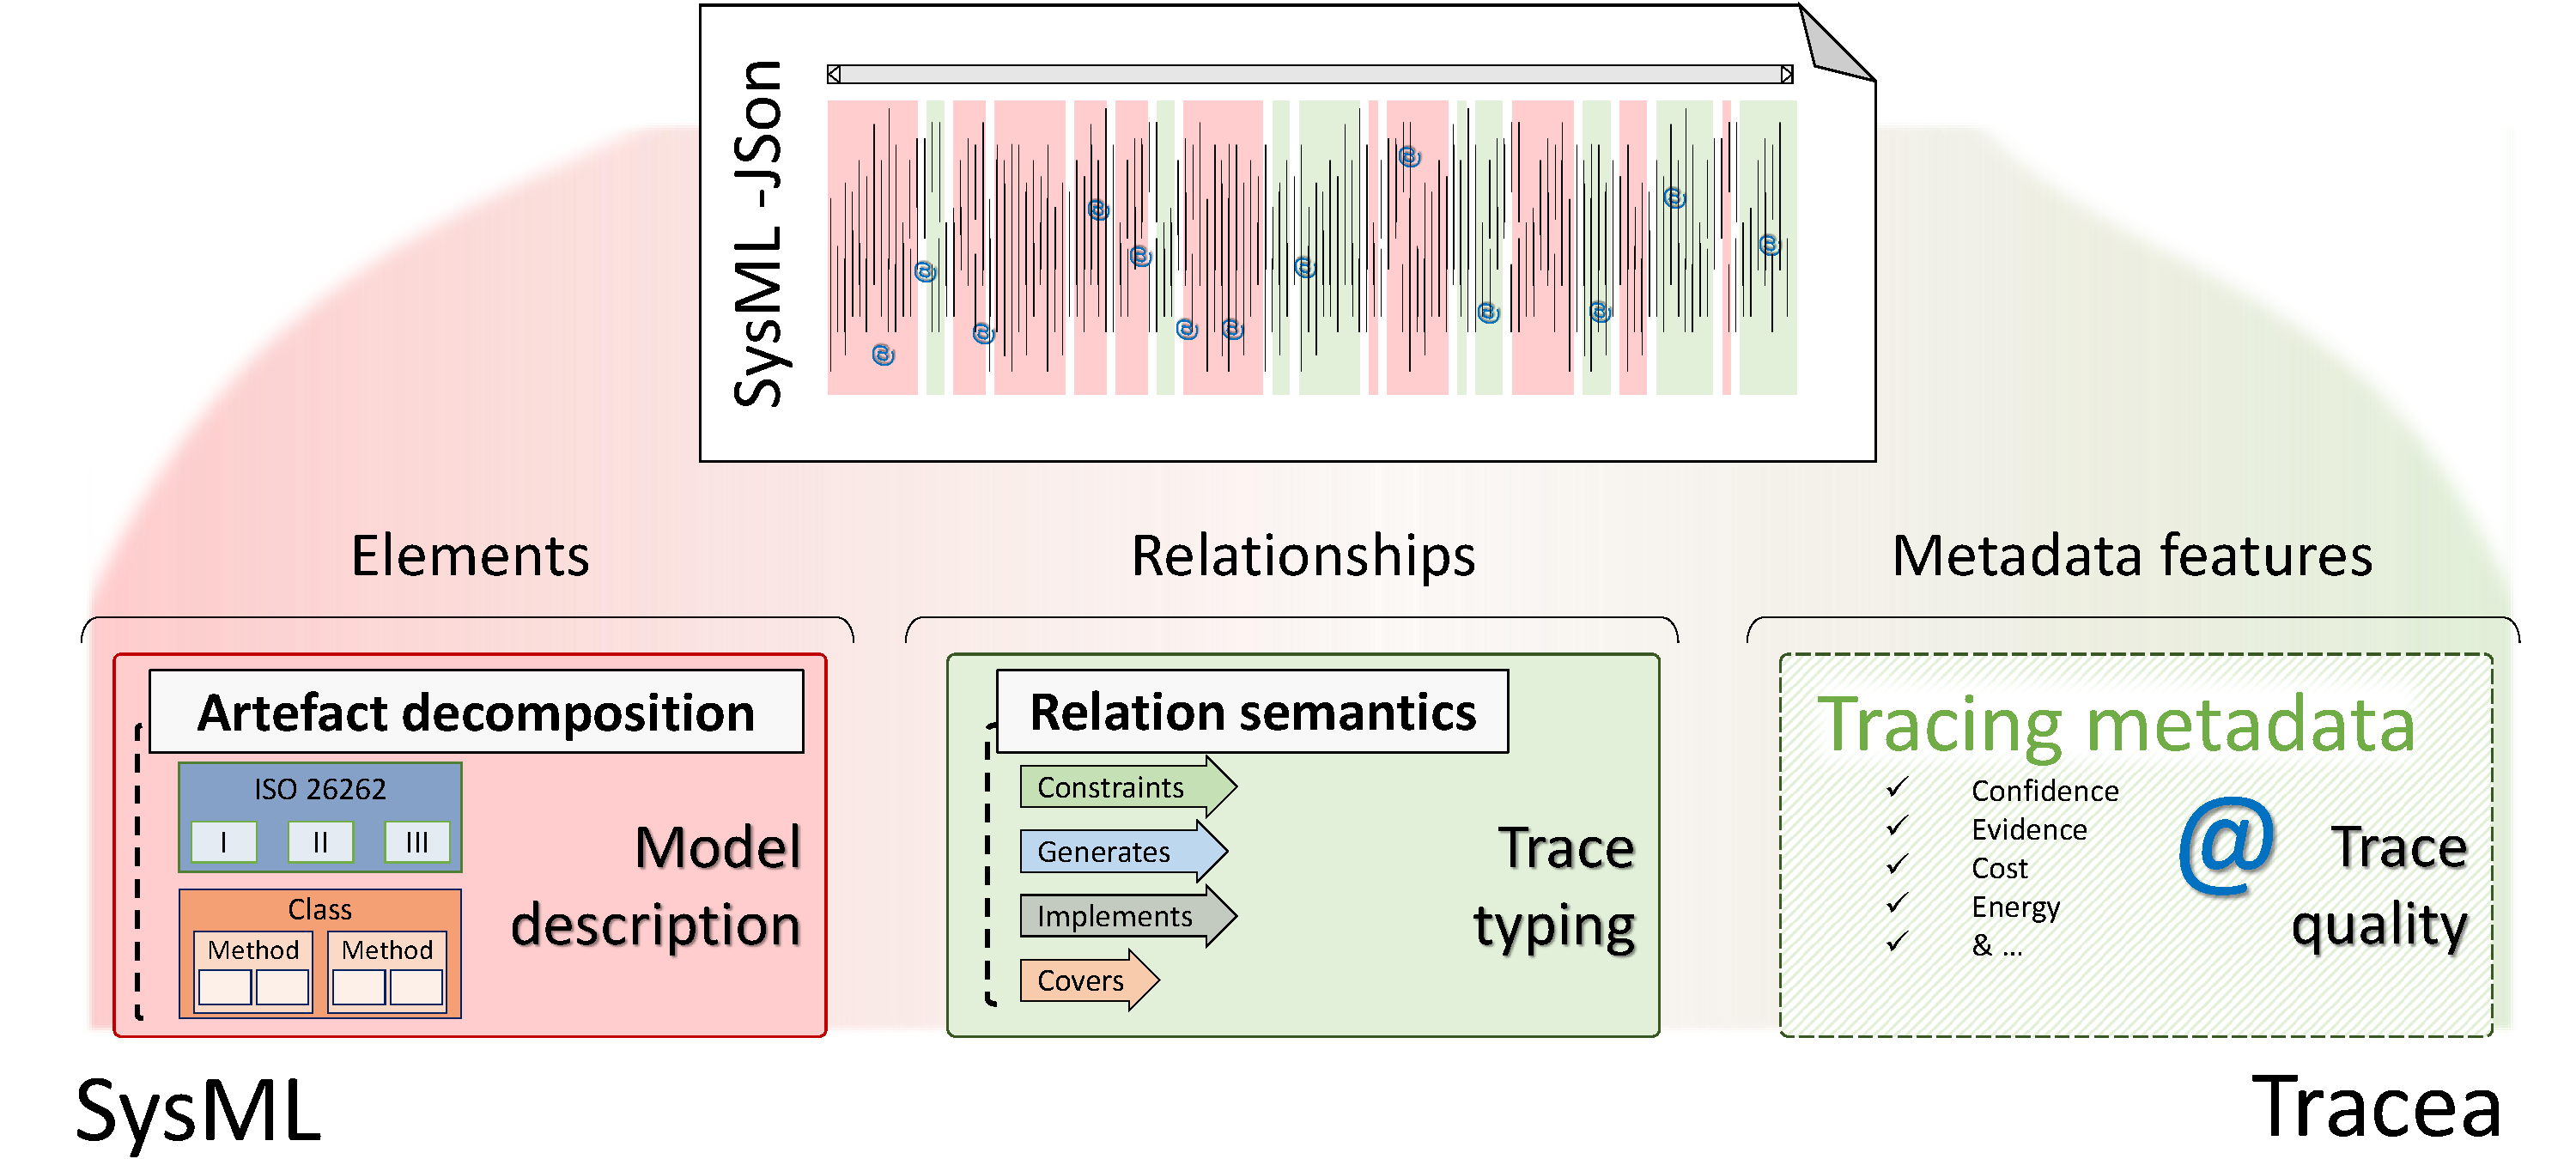
\includegraphics[width=.8\linewidth]{images/sysmljson-orga.pdf}
	\caption{Organisation of SysMLv2 JSon representation.}
	\label{fig:sysmljson-orga}
\end{figure}

% \begin{figure}[ht]     
% 	\centering
% 	\includegraphics[width=.7\linewidth]{images/cu-af-mf.jpg}
% 	\caption{Schematizing the multi-types conundrum.}
% 	\label{fig:multitypes}
% \end{figure}

\subsection{JSonTransformer: from SysMLv2 to TraceaML}
\begin{figure}[h]     
	\centering
	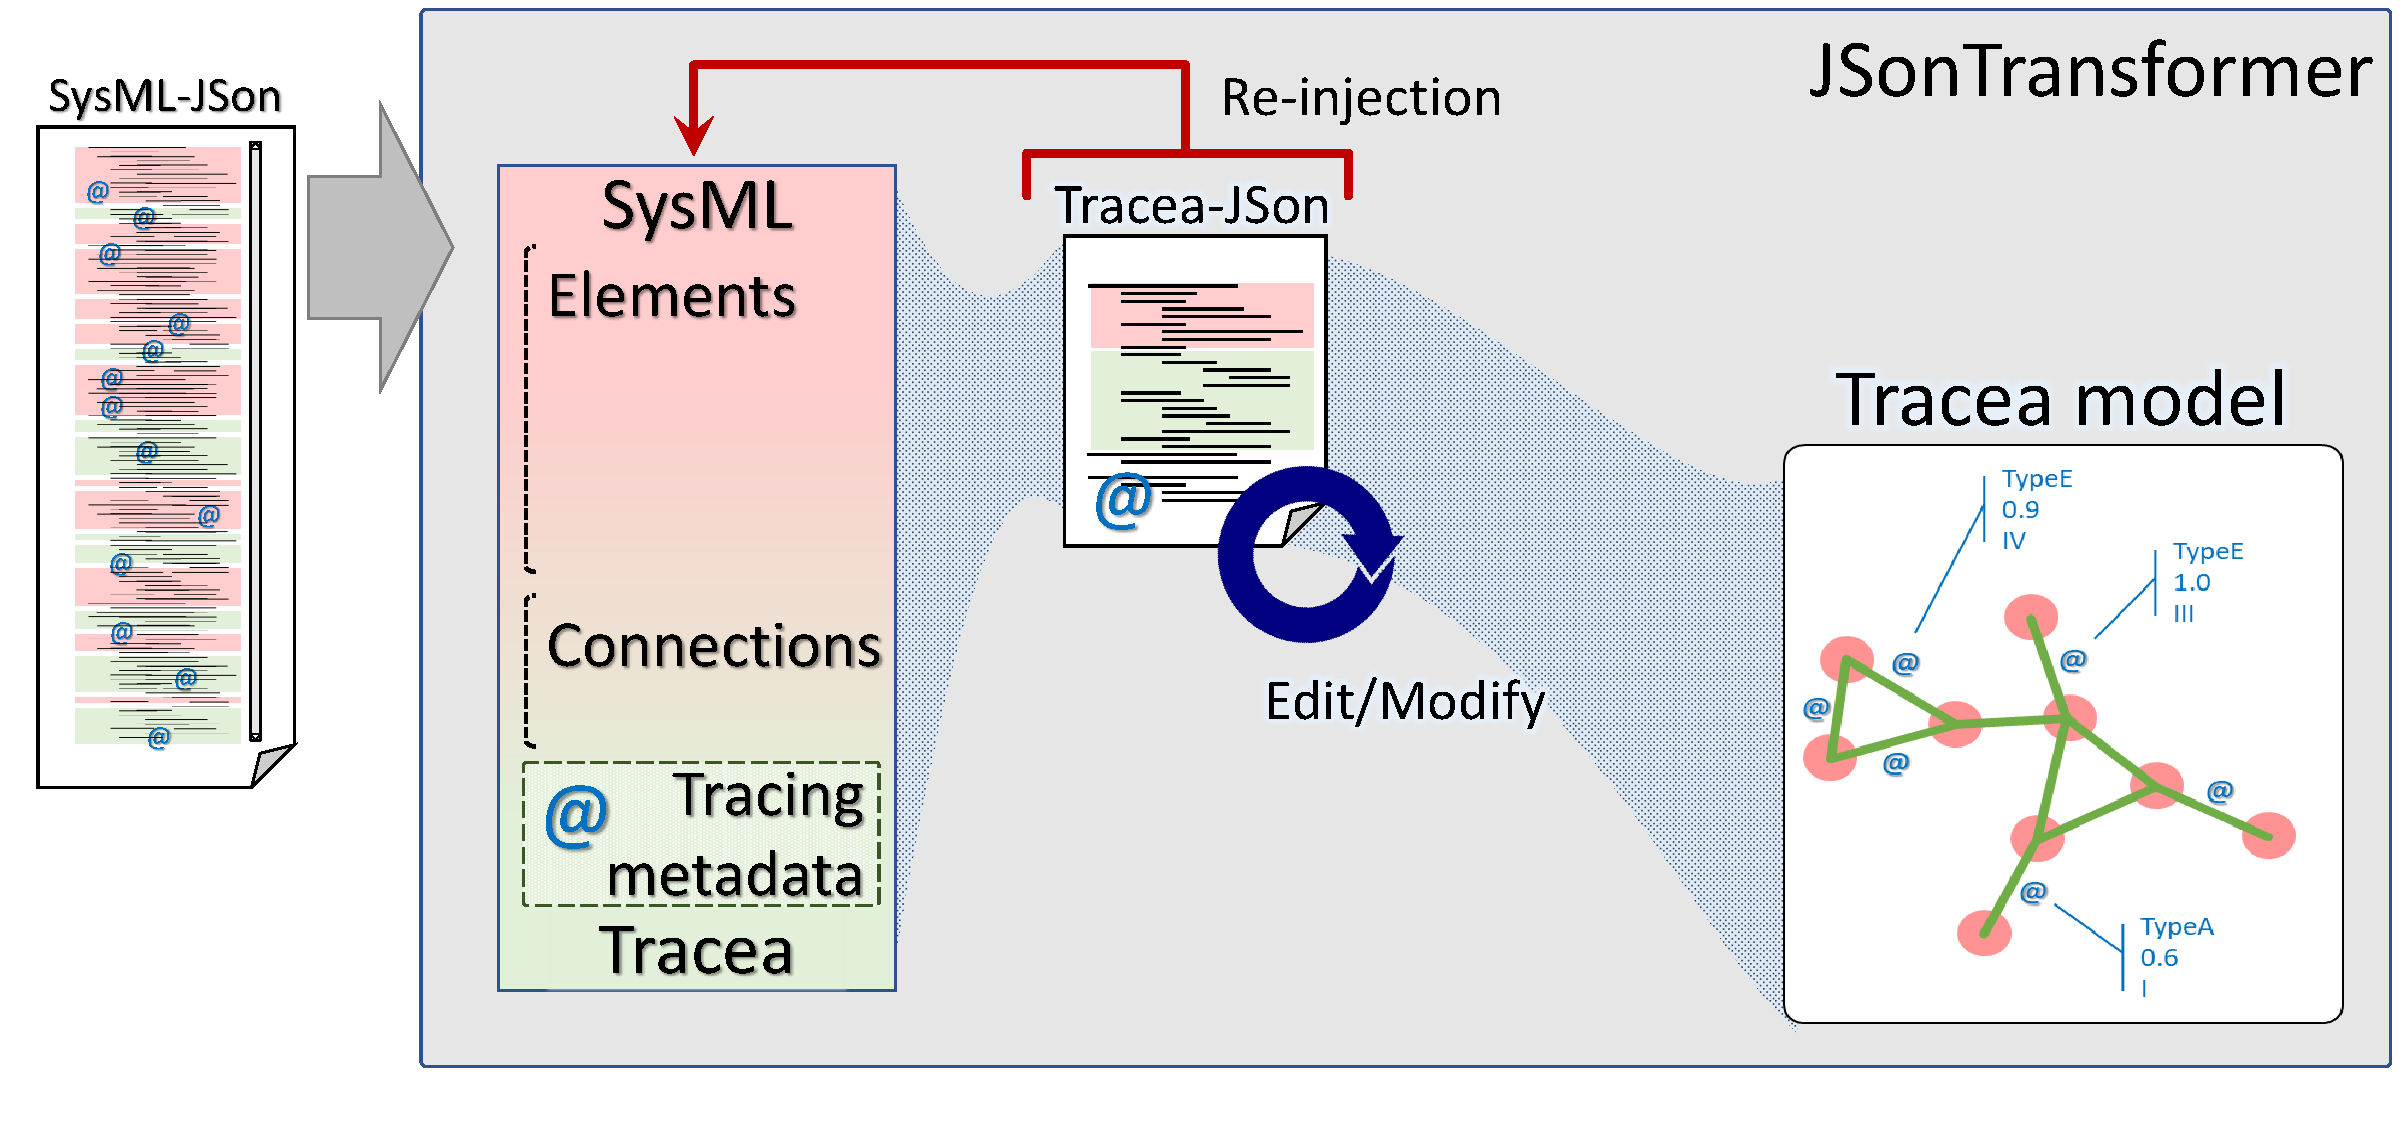
\includegraphics[width=.85\linewidth]{images/JSonTransformer-intern.pdf}
	\caption{JSonTransformer: integration of Tracea with SysMLv2.}
	\label{fig:jsontransformer}
\end{figure}

\Fig{fig:jsontransformer} shows the big picture of the integration of Tracea and SysMLv2 with JSonTransformer\footnote{\url{https://github.com/ebatot/TraceaingJson}}. To remain orthogonal to the system, and to asynch ourselves from the changes in the language itself, we export a JSon snapshots of the SysMLv2 model. Export can be made from the Jupyter implementation or the Eclipse pilot implementation independently. From this very voluble expression of the model (say 50kLoC for a minimalist model of a few elements and a couple of links), we extract a core model to transform and manipulate easily into other format (for more details about Tracea-JSon see Section~\ref{sec:traceamodel}). This format allows the use of multi-end and multi-type links, using the IDs of the elements in the same manner as the original (SysML) file. 

\textit{[Most of the work here lies in the transformation from this raw JSon to the prettied "Tracea" version we target.]}


\subsection{Extraction and re-injection of metadata}

\begin{figure}[ht]
	\centering
	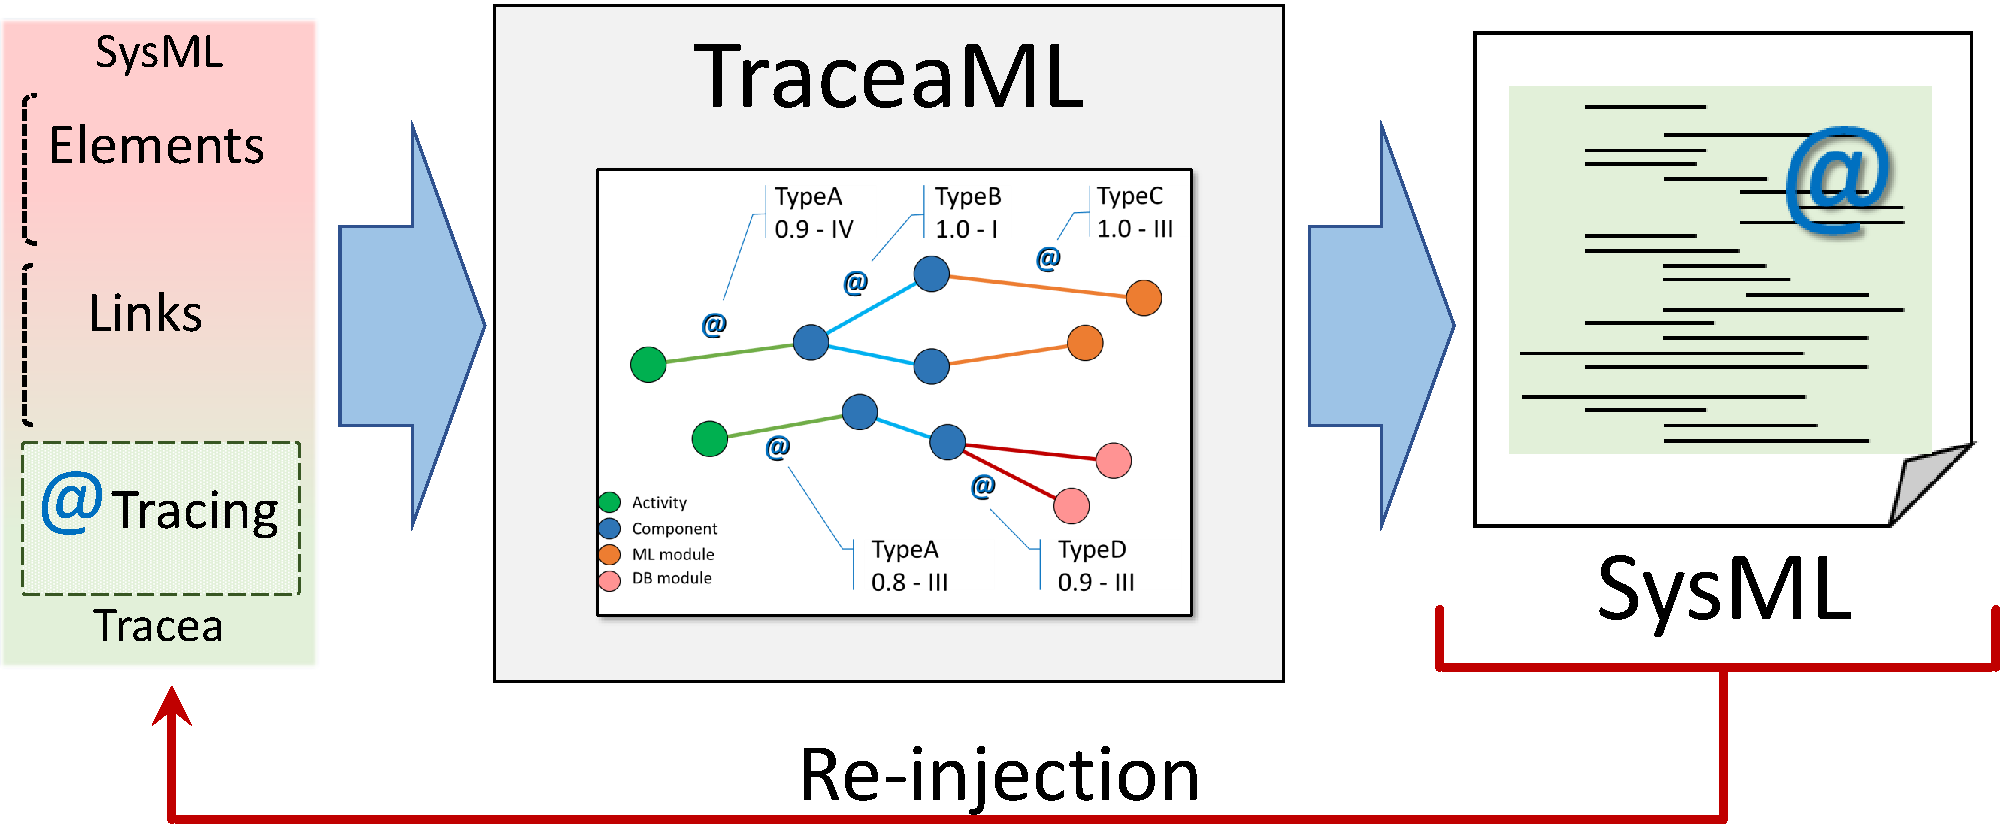
\includegraphics[width=.7\linewidth]{images/reinject.pdf}
	\caption{Re-injection of tracing metadata into a SysML model.}
	\label{fig:reinject}
\end{figure}

Transforming the JSon persistence of the SysMLv2 model comes at a cost. The entire JSon is used as input and our tool extract the necessary information. After editing this information, we re-inject it in the model through a (model-to-text) transformation. We take the \textit{Tracea} model and transform it to SysMLv2 textual notation. 

This method allows us to remain independent from the evolution of the pilot implementation. We act directly on the concrete artefacts -- which in the eyes of the SST is bond to its present version and will not change (\textit{much}) any soon. This method follows a bottom up understanding of the model: we reason from examples (at the instance level) to build and browse the feature paths of interest of the SysMLv2 metamodel. 

\subsection{Implementation details}

\subsubsection{Conditions of use}

Using a JSon snapshot requires that the instances of the links (or \textit{ConnectionUsages} in SysMLv2 terminology) be stored separately, and named. Indeed, metadata is affected to elements through their name. We only target (and source) tracelink with coarse grain elements to avoid the engineering complexity to browse feature paths. 
Summarized:
\begin{itemize}
    \item \textbf{Separated files} -- in order to re-inject the connections and their metadata, these must be kept separated in SysML (textual).
    \item \textbf{Named connections} -- metadata attribution from external source (the keyword "metadata" requires a named target).
    \item \textbf{Coarse grain targets} -- browsing features' path is a coding challenge on its own that is not addressed in the current version of our implementation.
    \item \textbf{External metadata} -- in order to be able to re-inject metadata without collision with existing ones, all metadata must be "external", \textit{i.e.,} declared with "metadata" keyword in SysML.
    \item \textbf{Feature IDs "bug"} -- Identification of SysMLv2 features is buggy: the same feature called from two connections distinct show two IDs. We bypass this limitation using names as identifier for features.
\end{itemize}

\subsubsection{Unexpected SysMLv2 identifier allocation}
As mentioned previously, implementing JSonTransformer, we ran into an unexpected behavior related to the allocation of identifiers to targets and sources of connections. We reported the "bug" to the SST and recorded it in our Git repository at \url{https://github.com/modelia/tracea/tree/master/4-sysml-json-transformer/sysml_id_allocation_bug}

\subsubsection{Programmatic version}

We envision a programmatic version of the current implementation. The use of the API in the pilot implementation has a steep learning curb and we opted in an hybrid version: using the JSon persistence of the models to work on propagation features. This way we work on concrete cases that we can craft to better suit our needs without requiring the actual implementation to be completely finished.

The current implementation will serve as a guide to implement a programmatic version. In this more interactive version, browsing elements will follow the exact same path as the JSon-snapshoted version.

\subsection{Summary}
\ugh{Need text !}
\Fig{fig:traceaml}  
\begin{figure}[h]     
	\centering
	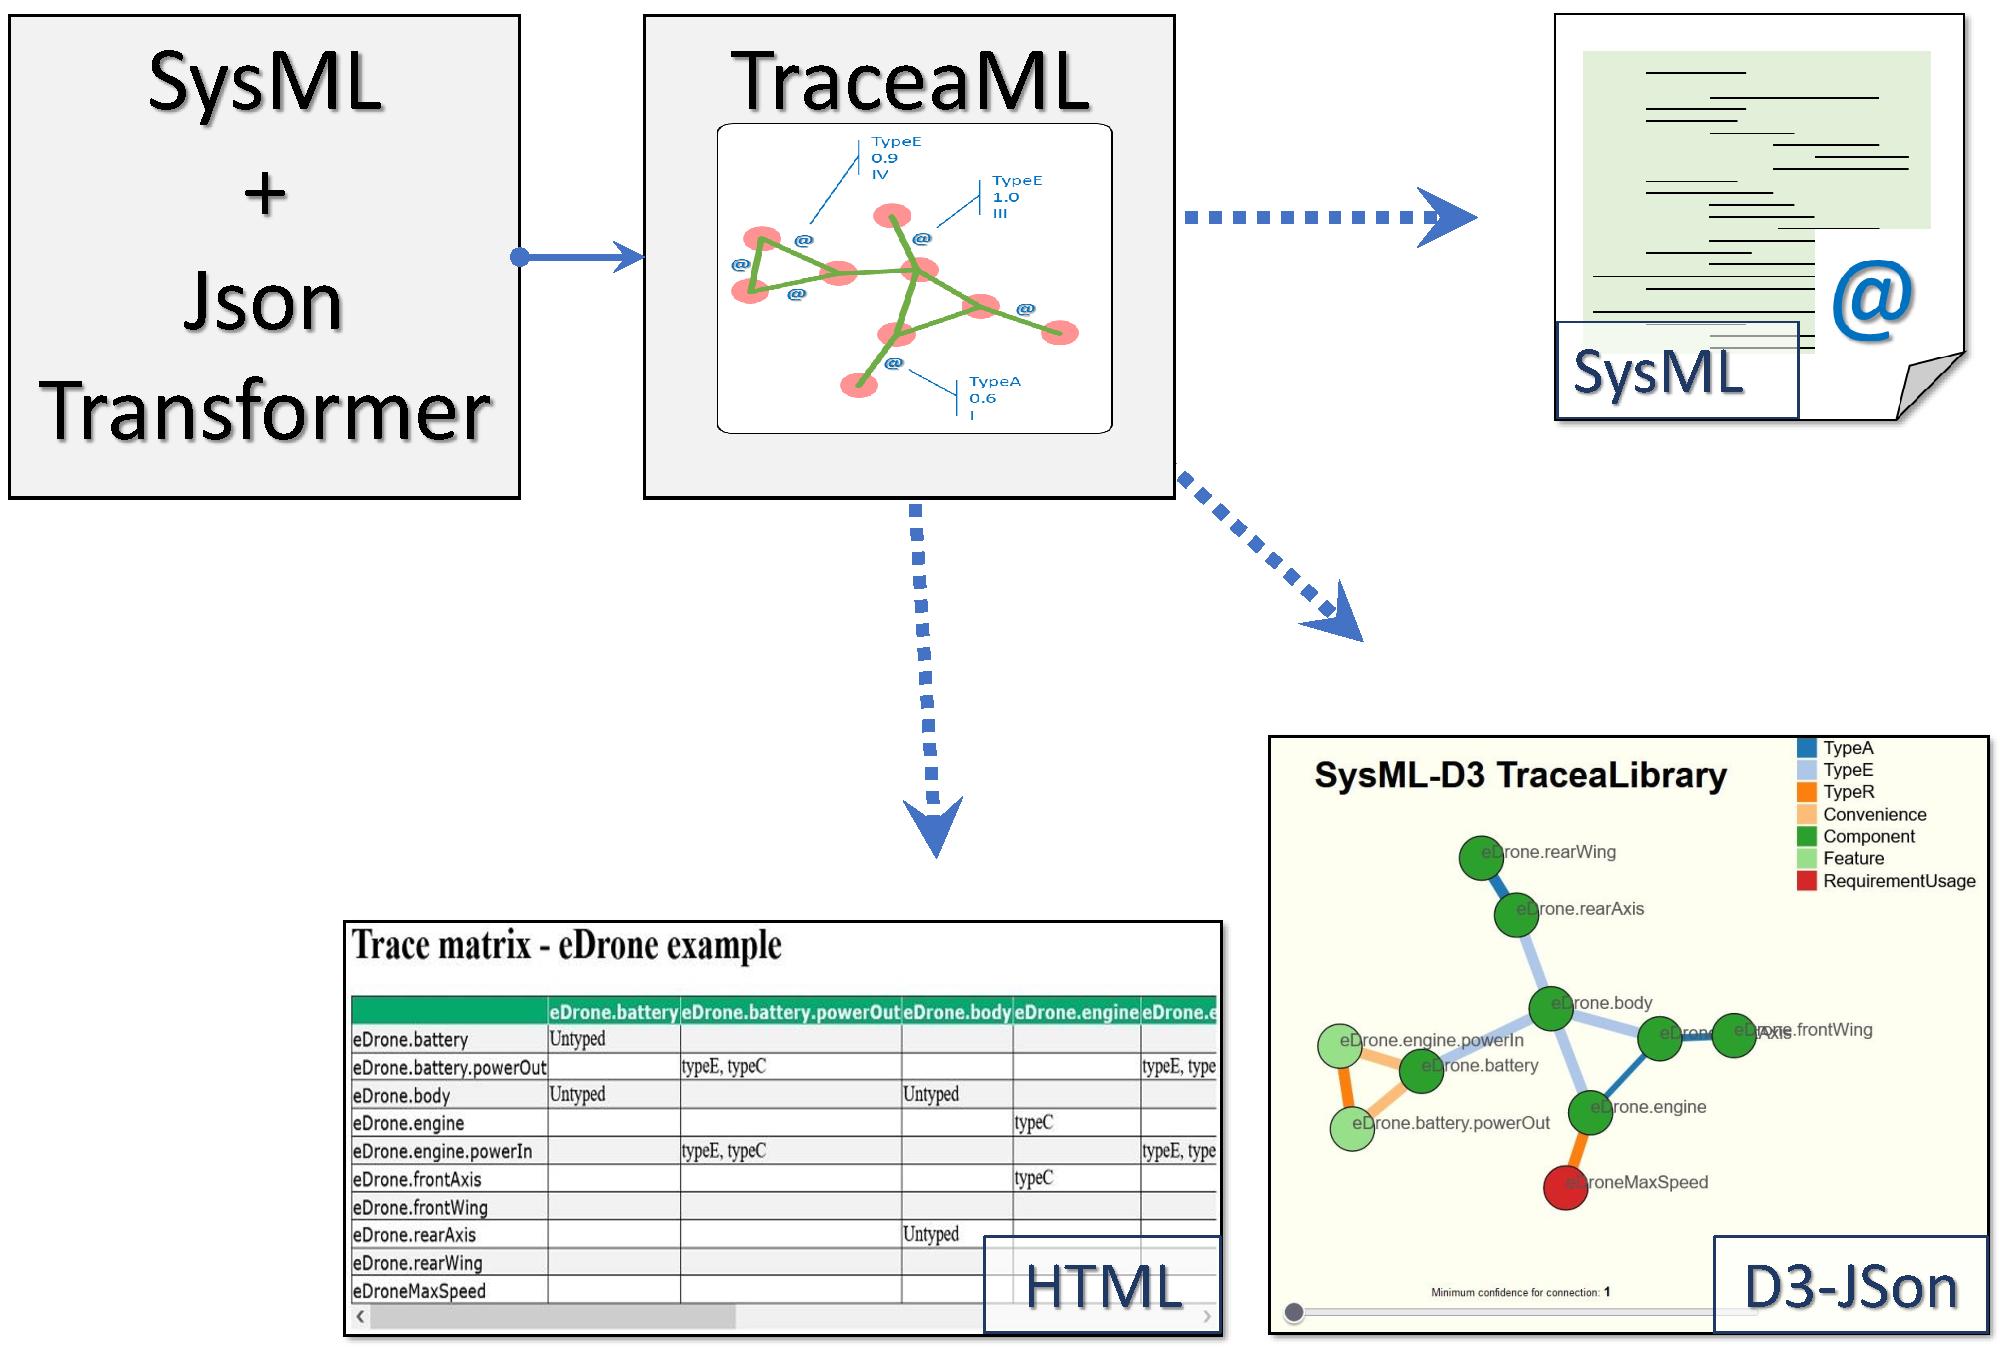
\includegraphics[width=.75\linewidth]{images/traceaml.pdf}
	\caption{SysMLv2 Tracing components, a big picture.}
	\label{fig:traceaml}
\end{figure}